\chapter{Computability and decidability}

\colorbox{green}{TEMPORARY - CM9}

\section{Computability and Turing machines}

\subsection{Definitions}
What computers can and can't do? \emph{Computability} answers this question.\\
There are problems no computer or algorithm can ever solve. This is a bad news.\\
To prove such results, we need a more formal definition of computations.

\begin{description}
\item[Intuitive definition of computing (Turing, 1936):] a human being is asked a \emph{question} ("input" or "instance", e.g. "123+479=?"), under the form of finitely many symbols from a finite alphabet, written on a sheet of paper.\\
The (human) computer can write down intermediate results, with unlimited supply of paper, using again symbols from a finite alphabet. The brain follows blindly, non-creatively, a finite list of elementary instructions. The next instruction is decided from the current instruction and the intermediate results currently under scruting by the computer on the paper.\\
There is an instruction called \texttt{STOP}. At this moment, the answer ("output") is written unambiguously on the paper (e.g."602 is the answer").

\item[Formal definition of computing (Turing, 1936):] a \emph{Turing machine} (T.M.) is composed of: 
\begin{itemize}
\item[$\bullet$] a \emph{tape}, which is bi-infinite, divided into cells, each being blank or containing a symbol from a finite alphabet $A$ (e.g. $A=\{0,1\}$);
\item[$\bullet$] a \emph{head}, which reads one cell at a time, can write a new symbol on this cell, shift the tape to the left or right.

\begin{center}
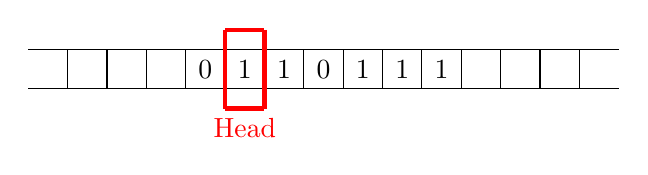
\begin{tikzpicture}
%horizontal lines
\draw (5,5)--(12.5,5);
\draw (5,4.5)--(12.5,4.5);

%vertical lines
\draw(5.5,5)--(5.5,4.5);
\draw(6,5)--(6,4.5);
\draw(6.5,5)--(6.5,4.5);
\draw(7,5)--(7,4.5);
\draw(7.5,5)--(7.5,4.5);
\draw(8,5)--(8,4.5);
\draw(8.5,5)--(8.5,4.5);
\draw(9,5)--(9,4.5);
\draw(9.5,5)--(9.5,4.5);
\draw(10,5)--(10,4.5);
\draw(10.5,5)--(10.5,4.5);
\draw(11,5)--(11,4.5);
\draw(11.5,5)--(11.5,4.5);
\draw(12,5)--(12,4.5);

%symbols
\node at (7.25,4.75) {$0$};
\node at (7.75,4.75) {$1$};
\node at (8.25,4.75) {$1$};
\node at (8.75,4.75) {$0$};
\node at (9.25,4.75) {$1$};
\node at (9.75,4.75) {$1$};
\node at (10.25,4.75) {$1$};

%head
\draw[color=red, ultra thick] (7.5, 5.25)--(7.5,4.25);
\draw[color=red, ultra thick] (8, 5.25)--(8,4.25);
\draw[color=red, ultra thick] (7.5, 5.25)--(8,5.25);
\draw[color=red, ultra thick] (7.5, 4.25)--(8,4.25);
\node[color=red] at (7.75,4) {Head};
\end{tikzpicture}
\end{center}

\item[$\bullet$] a finite set of instructions, each being numbered ($1,2,3,\hdots$) of the form: 
\begin{itemize}
\item[$\bullet$] \texttt{STOP}
\item[$\bullet$] "\texttt{if CurrentCell=blank/0/1}\\
\texttt{then Write(blank/0/1)}\\
\texttt{and ShiftLeft/ShiftRight/NoShift}\\
\texttt{and goto Instruction k.}"
\end{itemize}
\end{itemize}
So: \\
\begin{tabular}{ccccc}
\centering
&{\color{cyan}1936}&&{\color{cyan}$>$1948}&\\
\begin{tabular}{@{}c@{}}algorithm performed  \\ by a human brain \end{tabular} &{\color{cyan}\huge{$\leftrightarrow$}}&Turing machine&{\color{cyan}\huge{$\leftrightarrow$}}&modern computer\\
paper&{\color{cyan}\huge{$\leftrightarrow$}}&tape&{\color{cyan}\huge{$\leftrightarrow$}}&memory\\
(finite) brain&{\color{cyan}\huge{$\leftrightarrow$}}&head&{\color{cyan}\huge{$\leftrightarrow$}}&CPU\\
instructions&{\color{cyan}\huge{$\leftrightarrow$}}&instructions&{\color{cyan}\huge{$\leftrightarrow$}}&instructions, software\\
\end{tabular}
\end{description}

% \vspace{0.5cm}

A \emph{problem} $f$ is a (partial) mapping.
\begin{align*}
f:& A^*\rightarrow A^*\\
& w \rightarrow f(w) \text{ or undefined}\\
&\hspace*{-1cm} A=\text{ finite alphabet}\\
&\hspace*{-1cm}A^*=\text{ set of finite words, e.g. } A^*=\{\emptyset, 0, 1, 00, 01, 11, 10, 000, 001, \hdots\}\\
&\hspace*{-1cm}w=\text{ "input" or "instance"}\\
&\hspace*{-1cm}f(w)= \text{"output"}
\end{align*}

A problem $f$ is \emph{computed} or \emph{solved} by a Turing machine $T$ if whenever we write $w$ on an otherwise blank tape (and head is in initial instruction, at the beginning of $w$), $T$ runs and eventually stops if and only if $f(w)$ is defined, in which case the tape contains $f(w)$ only (if $f(w)$ is undefined, $T$ runs forever: infinite loop).\\

The problem $f$ is \emph{computable} if it is solved by at least a Turing machine.\\

A more \emph{modern machine} (Matlab machine): a Matlab machine is the code of a Matlab function (without "rand" instruction) running on an ideal infinite-memory computer.\\

\begin{theorem}
A problem is solved by a Turing machine if and only if it is solved by a Matlab machine.
\end{theorem}
\begin{proof}
\hfill
\begin{itemize}
\item[{\color{cyan}\fbox{$\Leftarrow$}}]  We have to convert any Matlab function into a T.M.=Matlab-to-TM compiler: admitted;
\item[{\color{cyan}\fbox{$\Rightarrow$}}] We have to write a TM-to-Matlab compiler: easier, admitted.
\end{itemize}
\end{proof}

We say that Matlab is "Turing-equivalent". So are Python, C, C$^{++}$ and Java.\\

\begin{thesis}[\textbf{Church-Turing}]
Any "obviously algorithmic" procedure (in the intuitive sense) corresponds to an equivalent T.M./Matlab program.
\end{thesis}
This is \emph{not} a theorem, because it is not formally defined. It is widely accepted because: 
\begin{itemize}
\item[$\bullet$] of Turing's argument about human computer;
\item[$\bullet$] every time we tried to convert an "obviously algorithmic" procedure into a T.M., we succeeded (with sweat and pain).\\
\end{itemize} 

It says for instance that the Euclidean division algorithm, "obviously algorithmic", can be solved by a T.M./a Matlab program (although the T.M. is not trivial to find).\\
Of course in this specific case we can prove formally that this T.M. exists, by constructing it.\\

With Church-Turing thesis, the theorem that Matlab is Turing-equivalent is trivial: Matlab instructions are clearly algorithmic.\\

Pay attention not confuse it with "strong Church-Turing thesis": anything the brain can do (writing poetry, proving theorems, ...) can be simulated by a T.M.\\
This one is highly controversial!\\

Now that we know what a formal algorithm is, we can prove \emph{theorems} about them.

\subsection{Universal Turing Machine}

\begin{theorem}[Turing, 1936]
The following problem is computable: 
\begin{itemize}
\item[$\bullet$] \emph{Input}: description of a T.M. ($T$) $+$ description of finite word on initial tape ("$w$");
\item[$\bullet$] \emph{Output}: \begin{itemize}
\item If $T$ stops when initial tape is $w$: \emph{the finite content of the tape};
\item If $T$ never stops: \emph{undefined}.
\end{itemize}
\end{itemize}

A T.M. solving it is called a "\emph{universal T.M.}".

\centering
\begin{tikzpicture}
%horizontal lines
\draw (5,10)--(12.5,10);
\draw (5,9.5)--(12.5,9.5);

%vertical lines
\draw(5.5,10)--(5.5,9.5);
\draw(6,10)--(6,9.5);
\draw(6.5,10)--(6.5,9.5);
\draw(7,10)--(7,9.5);
\draw(7.5,10)--(7.5,9.5);
\draw(8,10)--(8,9.5);
\draw(8.5,10)--(8.5,9.5);
\draw(9,10)--(9,9.5);
\draw(9.5,10)--(9.5,9.5);
\draw(10,10)--(10,9.5);
\draw(10.5,10)--(10.5,9.5);
\draw(11,10)--(11,9.5);
\draw(11.5,10)--(11.5,9.5);
\draw(12,10)--(12,9.5);

%head
\draw[color=red, ultra thick] (5.5, 10.25)--(5.5,9.25);
\draw[color=red, ultra thick] (6, 10.25)--(6,9.25);
\draw[color=red, ultra thick] (5.5, 10.25)--(6,10.25);
\draw[color=red, ultra thick] (5.5, 9.25)--(6,9.25);

% braces
\draw [decorate,decoration={brace,amplitude=6pt, mirror}] (5.5,9.25) -- (8.5,9.25) node [black,midway,yshift=-0.4cm] {\footnotesize description of $T$};
\draw [decorate,decoration={brace,amplitude=6pt, mirror}] (8.5,9.25) -- (12,9.25) node [black,midway,yshift=-0.4cm] {\footnotesize $w$};

%arrow
\begin{scope}[every edge/.append style = {snake arrow}]
\draw  (8.5,9) edge (8.5,6.25);
\end{scope}

%horizontal lines
\draw (5,6)--(12.5,6);
\draw (5,5.5)--(12.5,5.5);

%vertical lines
\draw(5.5,6)--(5.5,5.5);
\draw(6,6)--(6,5.5);
\draw(6.5,6)--(6.5,5.5);
\draw(7,6)--(7,5.5);
\draw(7.5,6)--(7.5,5.5);
\draw(8,6)--(8,5.5);
\draw(8.5,6)--(8.5,5.5);
\draw(9,6)--(9,5.5);
\draw(9.5,6)--(9.5,5.5);
\draw(10,6)--(10,5.5);
\draw(10.5,6)--(10.5,5.5);
\draw(11,6)--(11,5.5);
\draw(11.5,6)--(11.5,5.5);
\draw(12,6)--(12,5.5);

%head
\draw[color=red, ultra thick] (5.5, 6.25)--(5.5,5.25);
\draw[color=red, ultra thick] (6, 6.25)--(6,5.25);
\draw[color=red, ultra thick] (5.5, 6.25)--(6,6.25);
\draw[color=red, ultra thick] (5.5, 5.25)--(6,5.25);
% braces
\draw [decorate,decoration={brace,amplitude=6pt, mirror}] (5.5,5.25) -- (12,5.25) node [black,midway,yshift=-0.4cm] {\footnotesize $T(w)$};
\end{tikzpicture}

\end{theorem}
\begin{proof}
\hfill

\begin{itemize}
\item[$\bullet$] construct explicitely universal Turing Machine (thank you Alan)
\item[$\bullet$] OR construct explicitely universal Matlab machine.
\item[$\bullet$] OR by C-T thesis, simulating T is obviously algorithmic (in the intuitive sense) thus there is a Turing Machine doing it.
\end{itemize}
\end{proof}

\underline{NB:} Variante:\\
\begin{proof}
\hfill
\begin{itemize}
\item There's a Matlab program simulating any other Matlab program on any input.
\item There's a Turing Machine simulating any Matlab program on any input.\\
\begin{center}
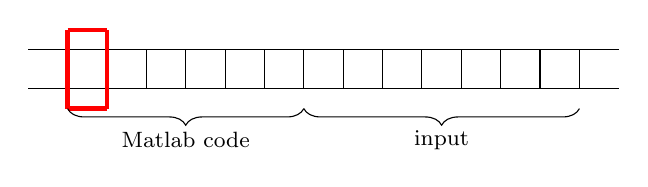
\begin{tikzpicture}
%horizontal lines
\draw (5,10)--(12.5,10);
\draw (5,9.5)--(12.5,9.5);

%vertical lines
\draw(5.5,10)--(5.5,9.5);
\draw(6,10)--(6,9.5);
\draw(6.5,10)--(6.5,9.5);
\draw(7,10)--(7,9.5);
\draw(7.5,10)--(7.5,9.5);
\draw(8,10)--(8,9.5);
\draw(8.5,10)--(8.5,9.5);
\draw(9,10)--(9,9.5);
\draw(9.5,10)--(9.5,9.5);
\draw(10,10)--(10,9.5);
\draw(10.5,10)--(10.5,9.5);
\draw(11,10)--(11,9.5);
\draw(11.5,10)--(11.5,9.5);
\draw(12,10)--(12,9.5);

%head
\draw[color=red, ultra thick] (5.5, 10.25)--(5.5,9.25);
\draw[color=red, ultra thick] (6, 10.25)--(6,9.25);
\draw[color=red, ultra thick] (5.5, 10.25)--(6,10.25);
\draw[color=red, ultra thick] (5.5, 9.25)--(6,9.25);

% braces
\draw [decorate,decoration={brace,amplitude=6pt, mirror}] (5.5,9.25) -- (8.5,9.25) node [black,midway,yshift=-0.4cm] {\footnotesize Matlab code};
\draw [decorate,decoration={brace,amplitude=6pt, mirror}] (8.5,9.25) -- (12,9.25) node [black,midway,yshift=-0.4cm] {\footnotesize input};
\end{tikzpicture}
\end{center}
\hspace*{7cm}=Matlab-to-TM \underline{interpreter}\\
\item Universal Turing Machine means that code is just data, written on memory, on the same level as the input.\\
\underline{e.g.}\\
\begin{center}
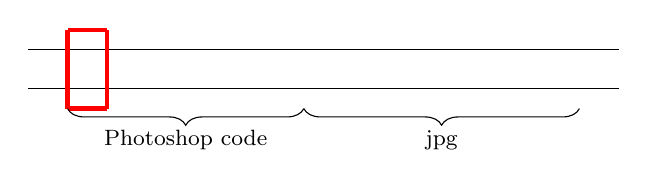
\begin{tikzpicture}
%horizontal lines
\draw (5,10)--(12.5,10);
\draw (5,9.5)--(12.5,9.5);


%head
\draw[color=red, ultra thick] (5.5, 10.25)--(5.5,9.25);
\draw[color=red, ultra thick] (6, 10.25)--(6,9.25);
\draw[color=red, ultra thick] (5.5, 10.25)--(6,10.25);
\draw[color=red, ultra thick] (5.5, 9.25)--(6,9.25);

% braces
\draw [decorate,decoration={brace,amplitude=6pt, mirror}] (5.5,9.25) -- (8.5,9.25) node [black,midway,yshift=-0.4cm] {\footnotesize Photoshop code};
\draw [decorate,decoration={brace,amplitude=6pt, mirror}] (8.5,9.25) -- (12,9.25) node [black,midway,yshift=-0.4cm] {\footnotesize jpg};
\end{tikzpicture}
\end{center}
\end{itemize}
\end{proof}
Modern computer are universal Turing Machines, i.e., they are (re-)programmable.\\
$\equiv$ Turing's fundamental insight.\\
(Pocket) 4-operation calculator = non universal T.M.

\section{Decidability}

\subsection{The Harting problem}
A decision problem is a total mapping: $A^*\rightarrow \{\text{YES,NO}\}$\\
E.g. "Is number $n$ prime?"\\
A decision problem is decidable if it's computable.\\

\underline{The Harting problem:}\\
\begin{leftbar}
Input:\begin{equation}
  \left\{
    \begin{split}
    \text{Matlab code f.m. + input for f}\\ 
    \text{ a T.M. description}
    \end{split}
  \right.
\end{equation}

Output:
\begin{itemize}
\item YES if f eventually stops on input x
\item NO if f never stops ("infinite loop")
\end{itemize}
\end{leftbar}